\section {Gather-Scatter-based Multi-leader all-to-all algorithm}
\subsection{Leader-based All-to-All Collective (L-a2a)}
In this section, we present the Leader-based all-to-all design.
Its algorithm is shown in Algorithm \ref{algorithm-node-aware}.



In algorithm \ref{algorithm-Leader-based}, the first step is a gathering procedure.
In each loop i, all message which need to be sent to node i are gathered into leader ranks of each node and transpose blocks sequentially.
The second step is a inter-node all-to-all between node-leaders.
In each loop i of the final step, messages which received from node i are scattered to the corresponding processes. 



\begin{algorithm}
 \caption{Leader-based All-to-All (L-a2a)}\label{algorithm-Leader-based}
\SetAlgoLined
\SetKwProg{Def}{def}{:}{}
\Def{All-to-all(SendBuf,RecvBuf,count,type,comm)}{
	\For{i in range(0,nodeN)}
	{
		Gather(SendBuf,gather\_result,intra\_node)\;
		transpose(gather\_result,BufferS)
	}
	\If{$myrank $==$ leader$}{Alltoall(BufferS,BufferR,inter\_node)}
	\For{i in range(0,nodeN)}
	{
		Scatter(BufferR,RecvBuf,intra\_node)
	}
}
\end{algorithm}
\begin{algorithm}
\caption{Leaders Placement of MPML}\label{Multi-leader-placement}
\SetKwProg{Def}{def}{:}{}
\Def{am-i-leader(intra-rank)}
{
	\If{intra-rank $<$ LeaderN}{
		return True
	}
	return False
}
\Def{my-leader-id(intra-rank)}
{
	return intra-rank
}
\end{algorithm}

The advantage of leader-based all-to-all collective are:
\begin{enumerate}[(1)]
\item Compared to direct all-to-all, leader-based  all-to-all reduce the number of message by $M^2$ time (M is the number of processes in each node). 
\item Similar to Bruck algorithm \cite{bruck1997efficient}, leader-based all-to-all aggregate the small message to large message. But leader-based all-to-all has less memory copy. It makes leader-based all-to-all suitable for medium-sized messages.
\end{enumerate}


\subsection{Multi-port Multi-leader All-to-all Collective (MPML)}
For larger messages, L-a2a involve too many intra-node overhead.
As a result, multiple network endpoints and processes can help to push the applicable boundary of gathering/scattering all-to-all futher away.
Multi-leader method is using multiple processes in a node to gather/scatter and transpose data.
Multi-port method is opening up multiple network endpoints by multiple processes which using multiple endpoints to process different communication requests.
MPML algorithm is shown in Algorithm \ref{Multi-leader-placement} and \ref{Multi-leader-based-a2a}  and Figure \ref{fig:MPML}.


\begin{algorithm}
\caption{Multi-port Multi-leader a2a (MPML)}\label{Multi-leader-based-a2a}
\SetAlgoLined
\KwIn{PPN:processes per-node, intra-rank: rank within a node, inter-rank: index of nodex
}
\SetKwProg{Def}{def}{:}{}

\Def {Multi-leader-gather(SendBuf,count)}
{
	MPI\_Win\_fence(intra-node)

	\If{am-i-leader(intra-rank)}
	{
		Lid = my-leader-id(intra-rank)

		\For{i in range(Lid,nodeN,LeaderN)}
		{
			target-node $\leftarrow$ (inter-rank + i) mod nodeN

			k $\leftarrow$ $\frac{i}{LeaderN}$

			shift $\leftarrow$ target-node*count*PPN

			\For {j in range(0,PPN)}
			{
				source $\leftarrow$ (intra-rank + j) mod P

				Get(gatherbuf[k][source],source,shift)
			}
			% 
		}
	}
	MPI\_Win\_fence(intra-node)
		
	Leaders transpose all blocks to BufferS
}
\Def {Multi-port-a2a(BufferS,BufferR)}
{
	\If{am-i-leader(intra-rank)}
	{
		Lid = my-leader-id(intra-rank)

		\For{i in range(Lid,nodeN,LeaderN)}
		{
			k $\leftarrow$ $\frac{i}{LeaderN}$

			target $\leftarrow$  (inter-rank + i) mod nodeN

			source $\leftarrow$  (inter-rank + nodeN - i) mod nodeN

			MPI\_Isend(BufferS[k],target)

			MPI\_Recv(BufferR[k],source)
		}

	}
	
}
\Def {Multi-leader-scatter(Recvbuf,count)}
{
	MPI\_Win\_fence(intra-node)

	\If{am-i-leader(intra-rank)}
	{
		Lid = my-leader-id(intra-rank)

		\For{i in range(Lid,nodeN,LeaderN)}
		{
			source-node $\leftarrow$ (inter-rank + nodeN - i) mod nodeN

			k $\leftarrow$ $\frac{i}{LeaderN}$

			shift $\leftarrow$ source-node*count*PPN

			\For {j in range(0,PPN)}
			{
				target $\leftarrow$ (intra-rank + j) mod P

				Put(BufferR[k][target],target,shift)
			}

		}
	}

	MPI\_Win\_fence(intra-node)
}
\Def{all-to-all(SendBuf,RecvBuf,count,type,comm)}{
	Multi-leader-gather(SendBuf,count,gatherbuf)

	Multi-port-a2a(BufferS,BufferR)

	Local-Transpose(BufferR)
	
	Multi-leader-scatter(Recvbuf,count)
}
\end{algorithm}

\begin{figure}
\centering
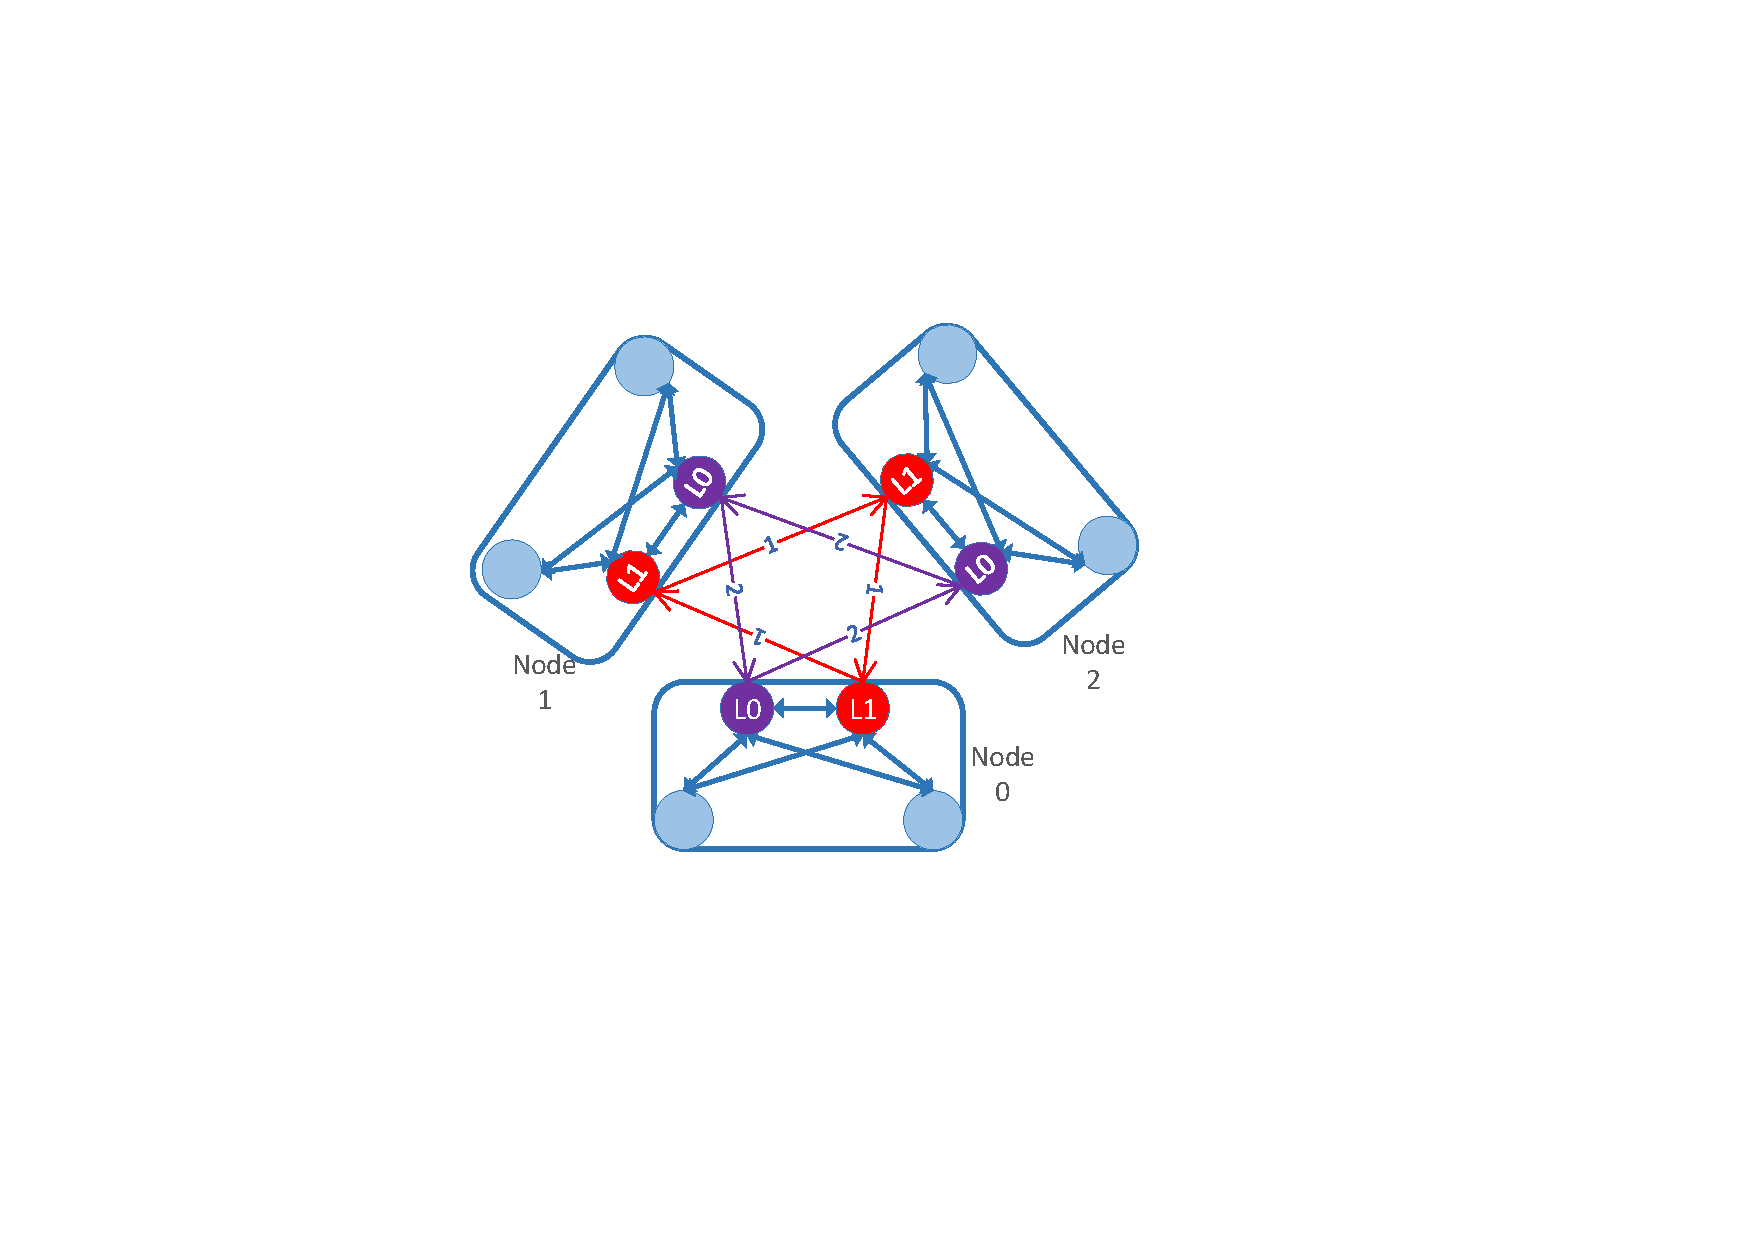
\includegraphics[width=8cm]{./Figures/multi-leader-multi-port-a2a.pdf} %[图片大小]{图片路径}
\caption{Example of 3 nodes 12 processes 2-leader MPML} %图片标题
\label{fig:MPML}
\end{figure}
As shown in Figure \ref{fig:MPML}, there are 2 leaders in a node, different processes are responsible for communicating with different nodes in a round-robin way.
Assume node A send a aggregated message to Node B where B equal to (A + i) mod NodeN.
Leaders i in node A and B are responsible for send and recv the message.


Compared to L-a2a, MPML takes advantage of multi-leader and multi-port to optimize L-a2a.
As disscussed in Motivation part, using multiple processes can improving the gathering and scattering throughput a lot in all message size and HPC we tested. 
Besides, using multiple processes to transpose the local blocks can parallise the local stransposing processes.
Multiple network endpoints can parallelize the startup overhead of multiple communication requests.


% \begin{figure}
% \centering
% % \subfigure[Example of 3 nodes 4 processes L-a2a]{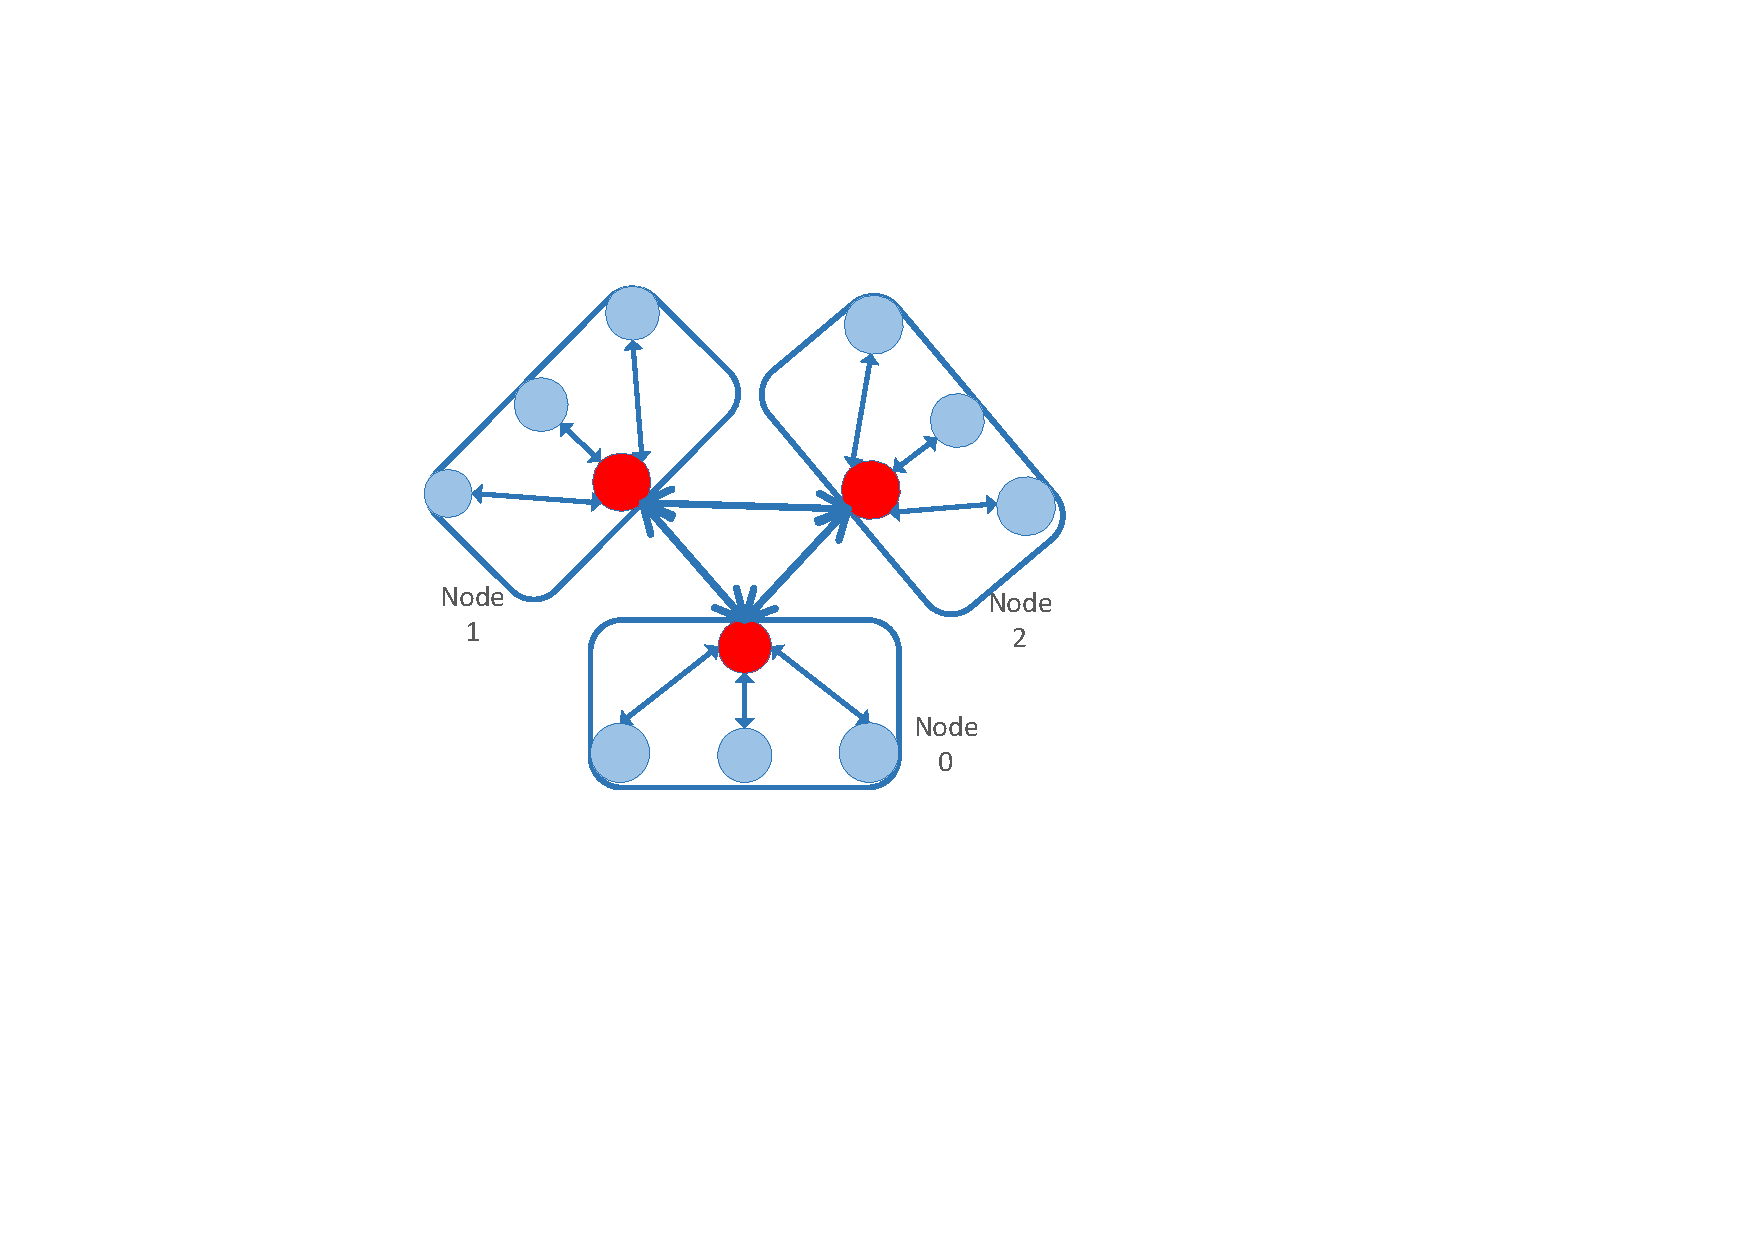
\includegraphics[width=4cm]{./Figures/leader-based-a2a.pdf}}
% \subfigure[Example of 3 nodes 4 processes MPML]{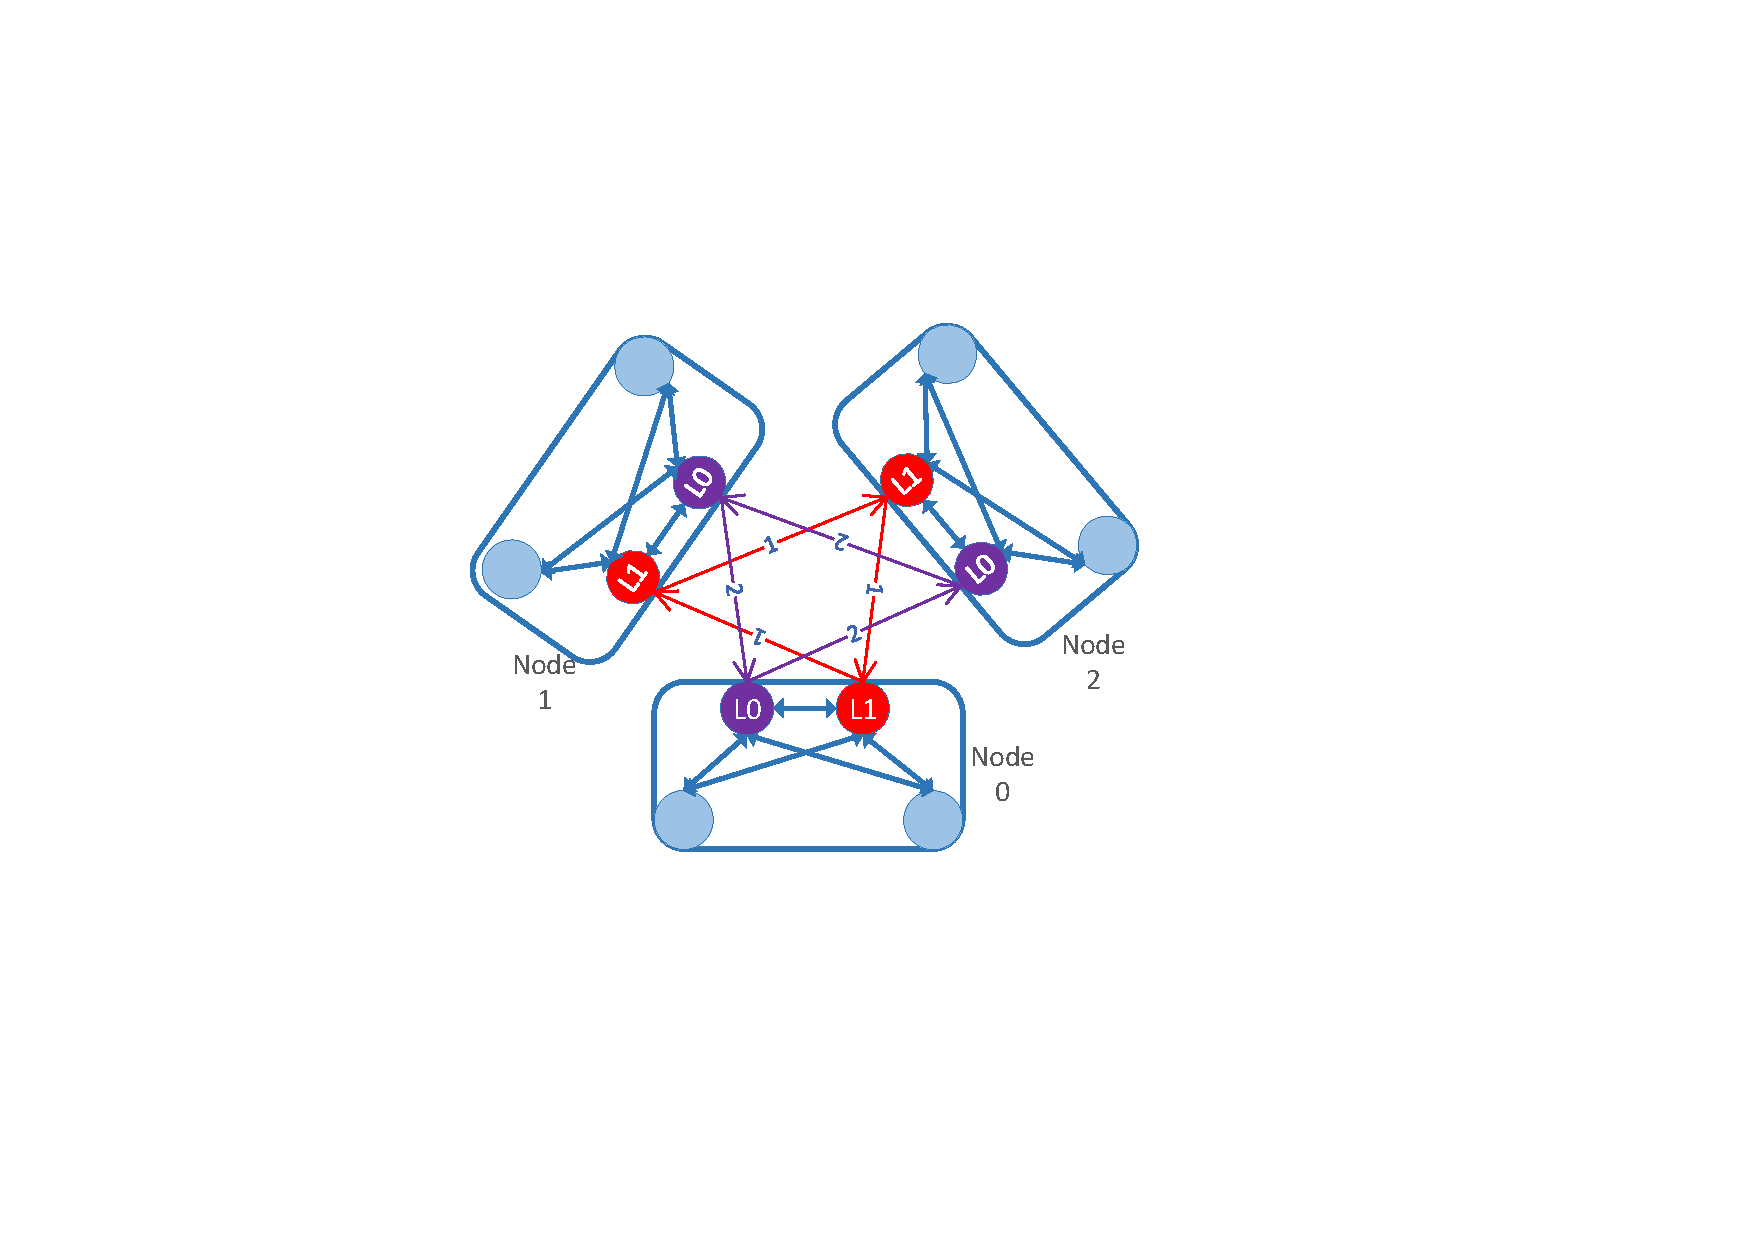
\includegraphics[width=8cm]{./Figures/multi-leader-multi-port-a2a.pdf}}
% % \caption{Jackson Yee} %图片标题
% \label{fig:1}  %图片交叉引用时的标签
% \end{figure}

\subsection {NUMA-aware MPML all-to-all collective (NMPML)}
There are usually NUMA architecture on mordern multi-core processes on supercomputers.
As different CPU has different count of NUMA.
We uniformly spread the leaders on a node to make them utilize all NUMAs.
The core idea can be shown as Figure \ref{fig:NUMA-Aware}.
\begin{figure}
\centering
\subfigure[4 leaders on a 4 NUMA 16 core processor]{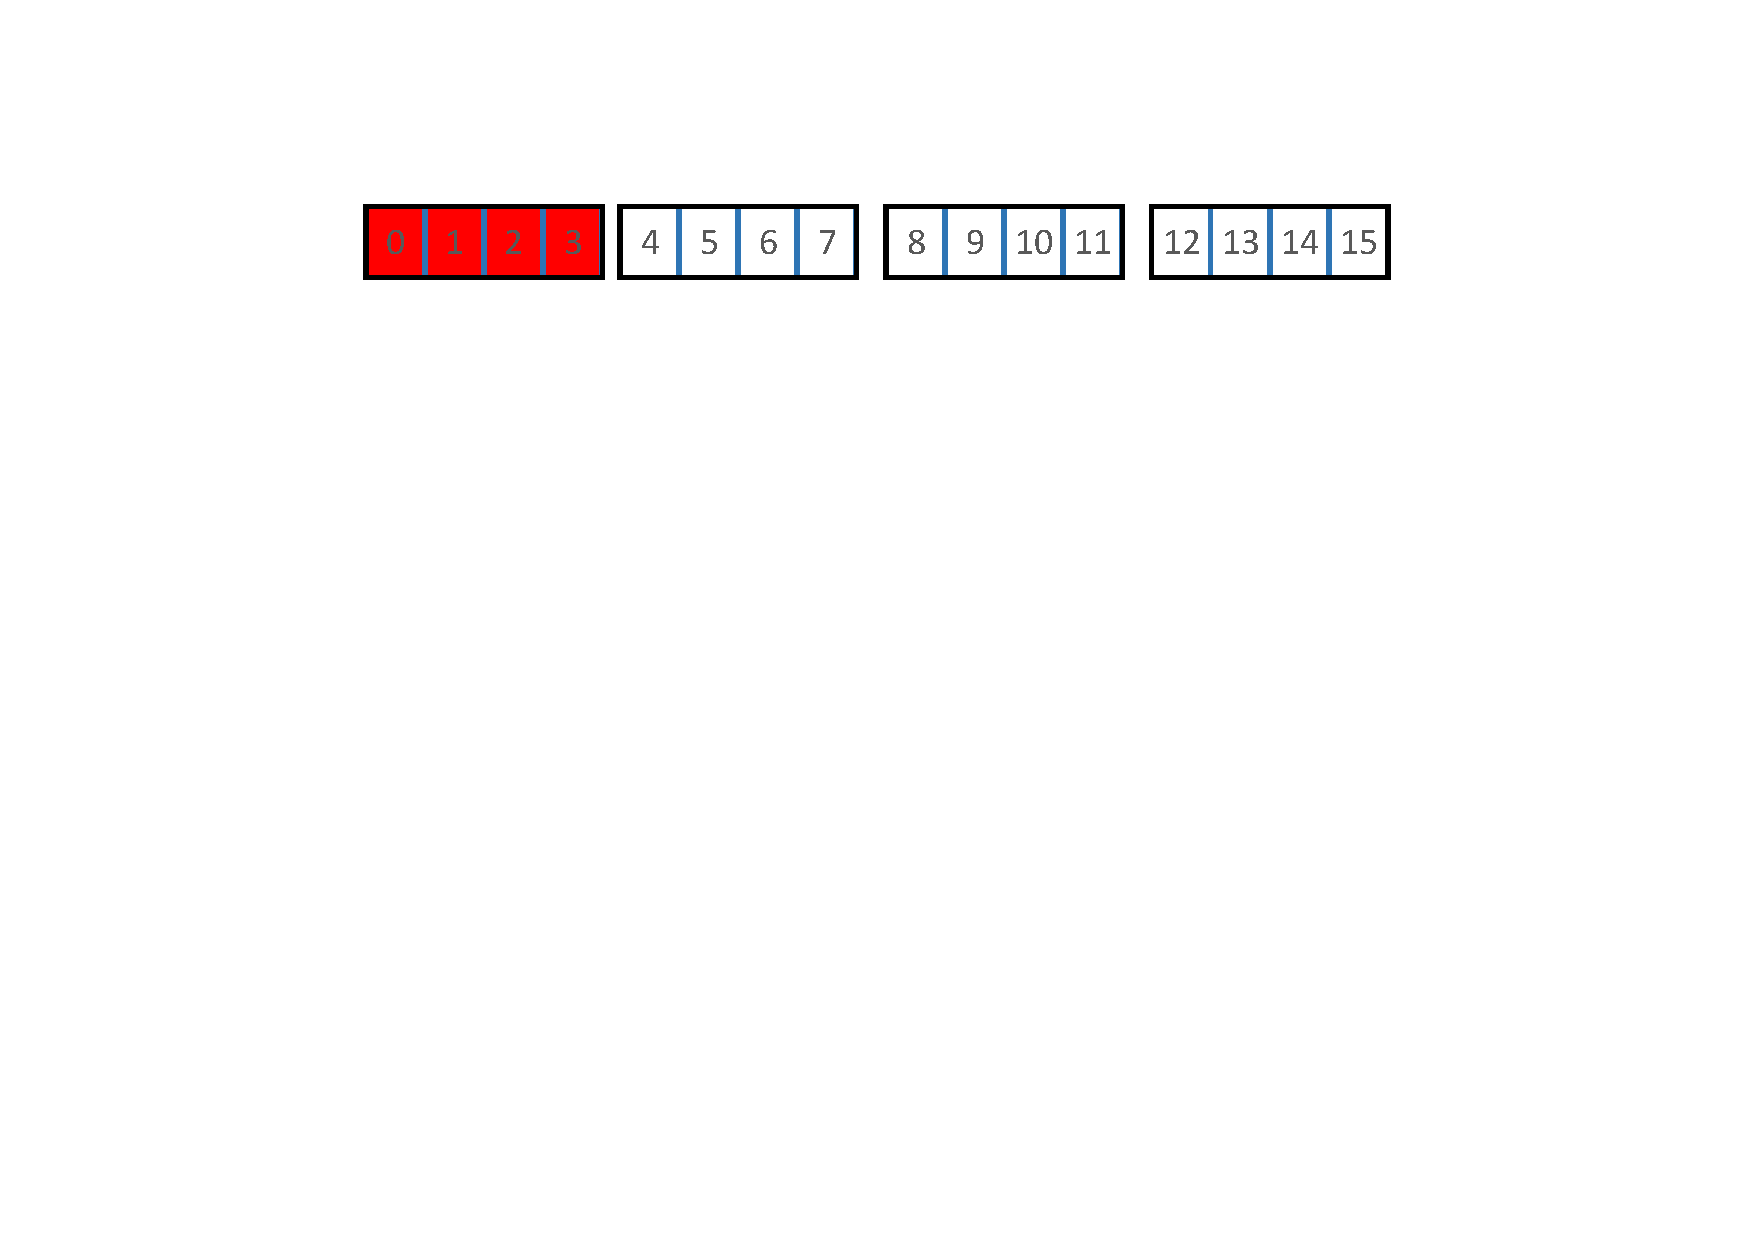
\includegraphics[width=8cm]{./Figures/no-NUMA-awarea2ax.pdf}}
\\
\centering
\subfigure[spreaded 4 leaders on a 4 NUMA 16 core processor]{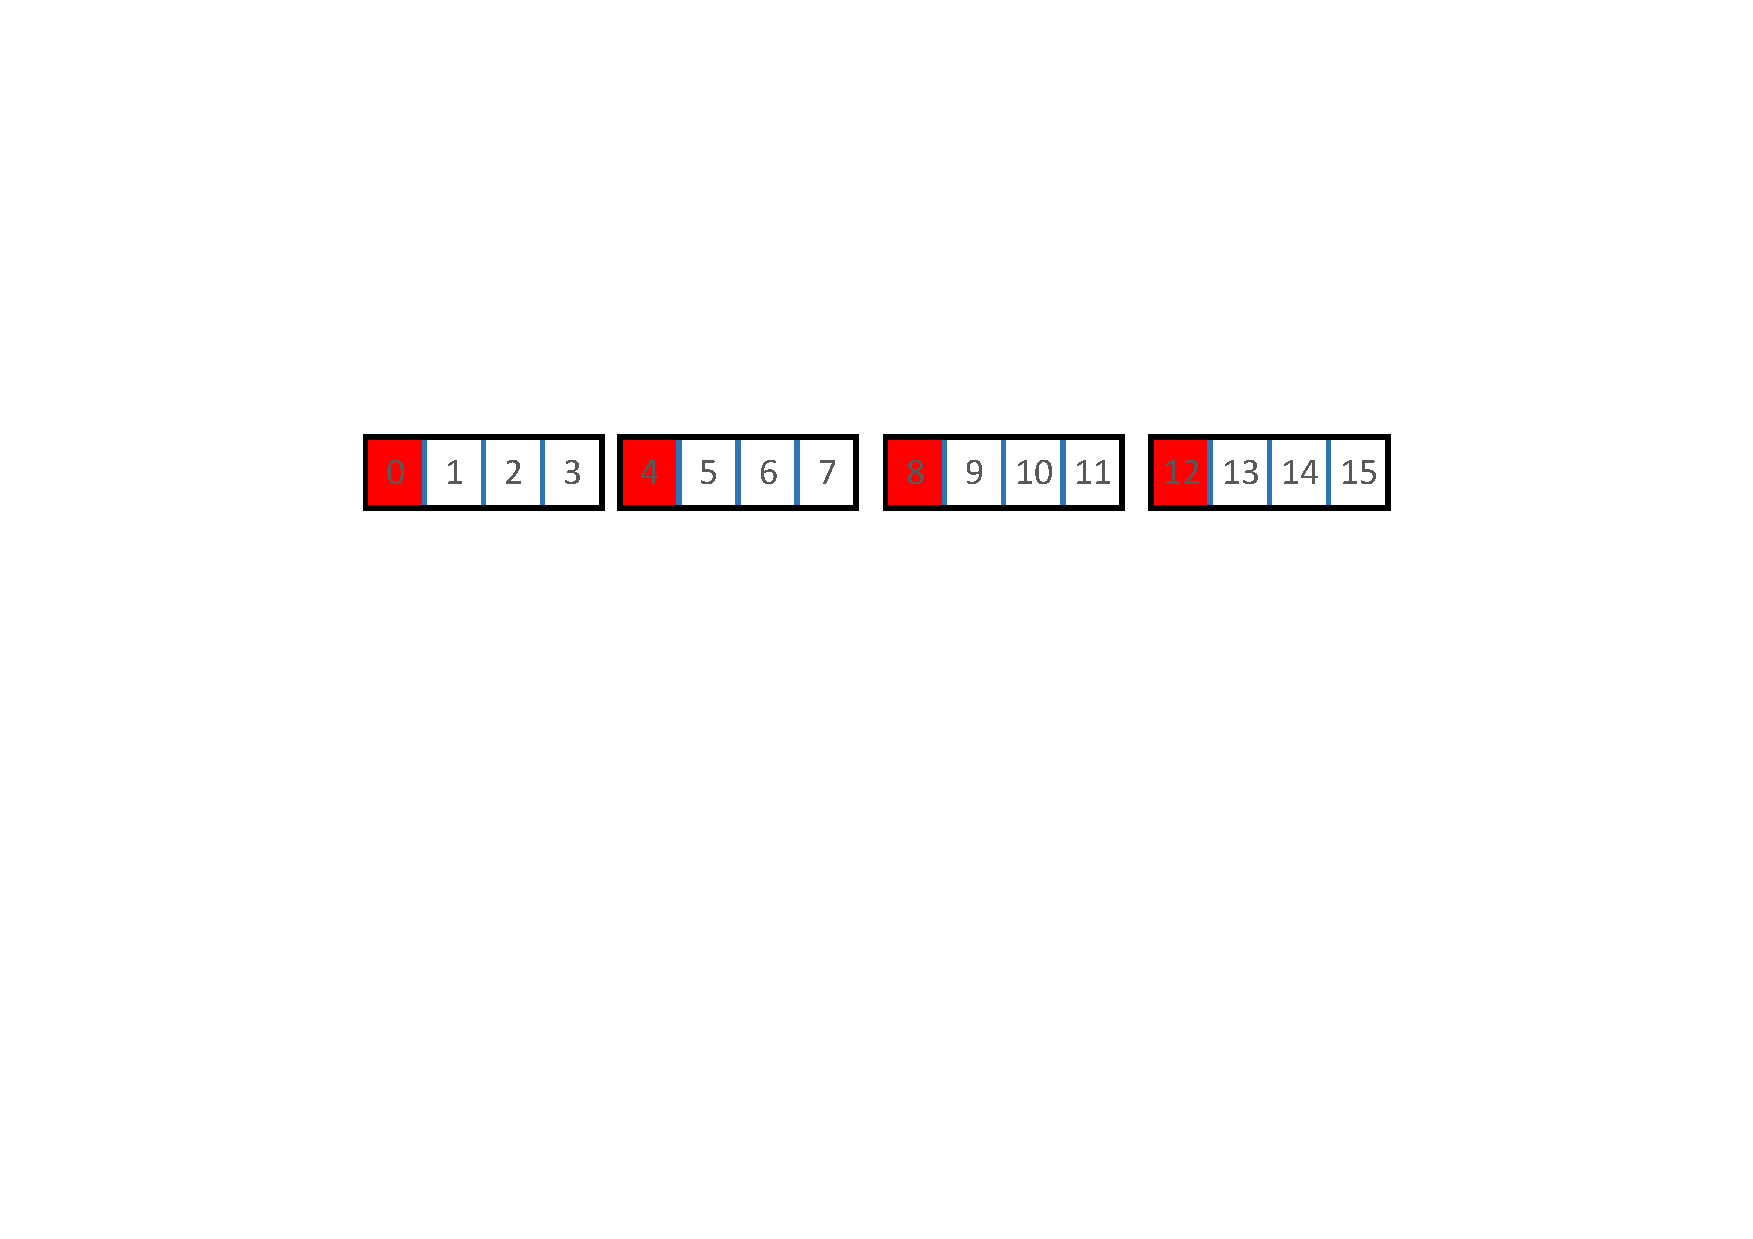
\includegraphics[width=8cm]{./Figures/NUMA-awarea2a.pdf}}
% \caption{Jackson Yee} %图片标题
\caption{NUMA-aware leader placement.} %图片标题
\label{fig:NUMA-Aware}  %图片交叉引用时的标签
\end{figure}

From algorithm view, the only difference between NMPML and MPML is the am-i-leader and my-leader-id functions.
In NMPML, we only to replace the Algorithm \ref{Multi-leader-placement} into Algorithm \ref{NMPML-Multi-leader-placement}.
\begin{algorithm}
\caption{Leaders Placement of NMPML}\label{NMPML-Multi-leader-placement}
\SetKwProg{Def}{def}{:}{}
\Def{am-i-leader(intra-rank)}
{
	dist $\leftarrow$  max($\lfloor \frac{intra-procn}{leaderN} \rfloor$, 1) \\
	t $\leftarrow \frac{intra-rank}{dist}$ \\
	r $\leftarrow$ intra-rank mod dist \\
	\If{r == 0 and t $<$ leaderN}{ 
		return True
	}
	return False
}
\Def{my-leader-id(intra-rank)}
{
	dist $\leftarrow$  max($\lfloor \frac{intra-procn}{leaderN} \rfloor$, 1) \\
	return $\frac{intra-rank}{dist}$
}
\end{algorithm}

As we have discussed in Motivation section, when spreading leaders on the node, we acquire beter gathring/scattering throughput in most cases.

\subsection{Overlapping Intra-node and Inter-node Communication of NMPML (ONMPML)}


We notice that the overead of gathering, scattering, and transpose can be overlapped with inter-node communication.
As shown in Figure \ref{fig:ONMPML}, there are 2 leaders in a node. 
Each leaders send a block immediately after the block is gathered.
\begin{figure*}
\centering
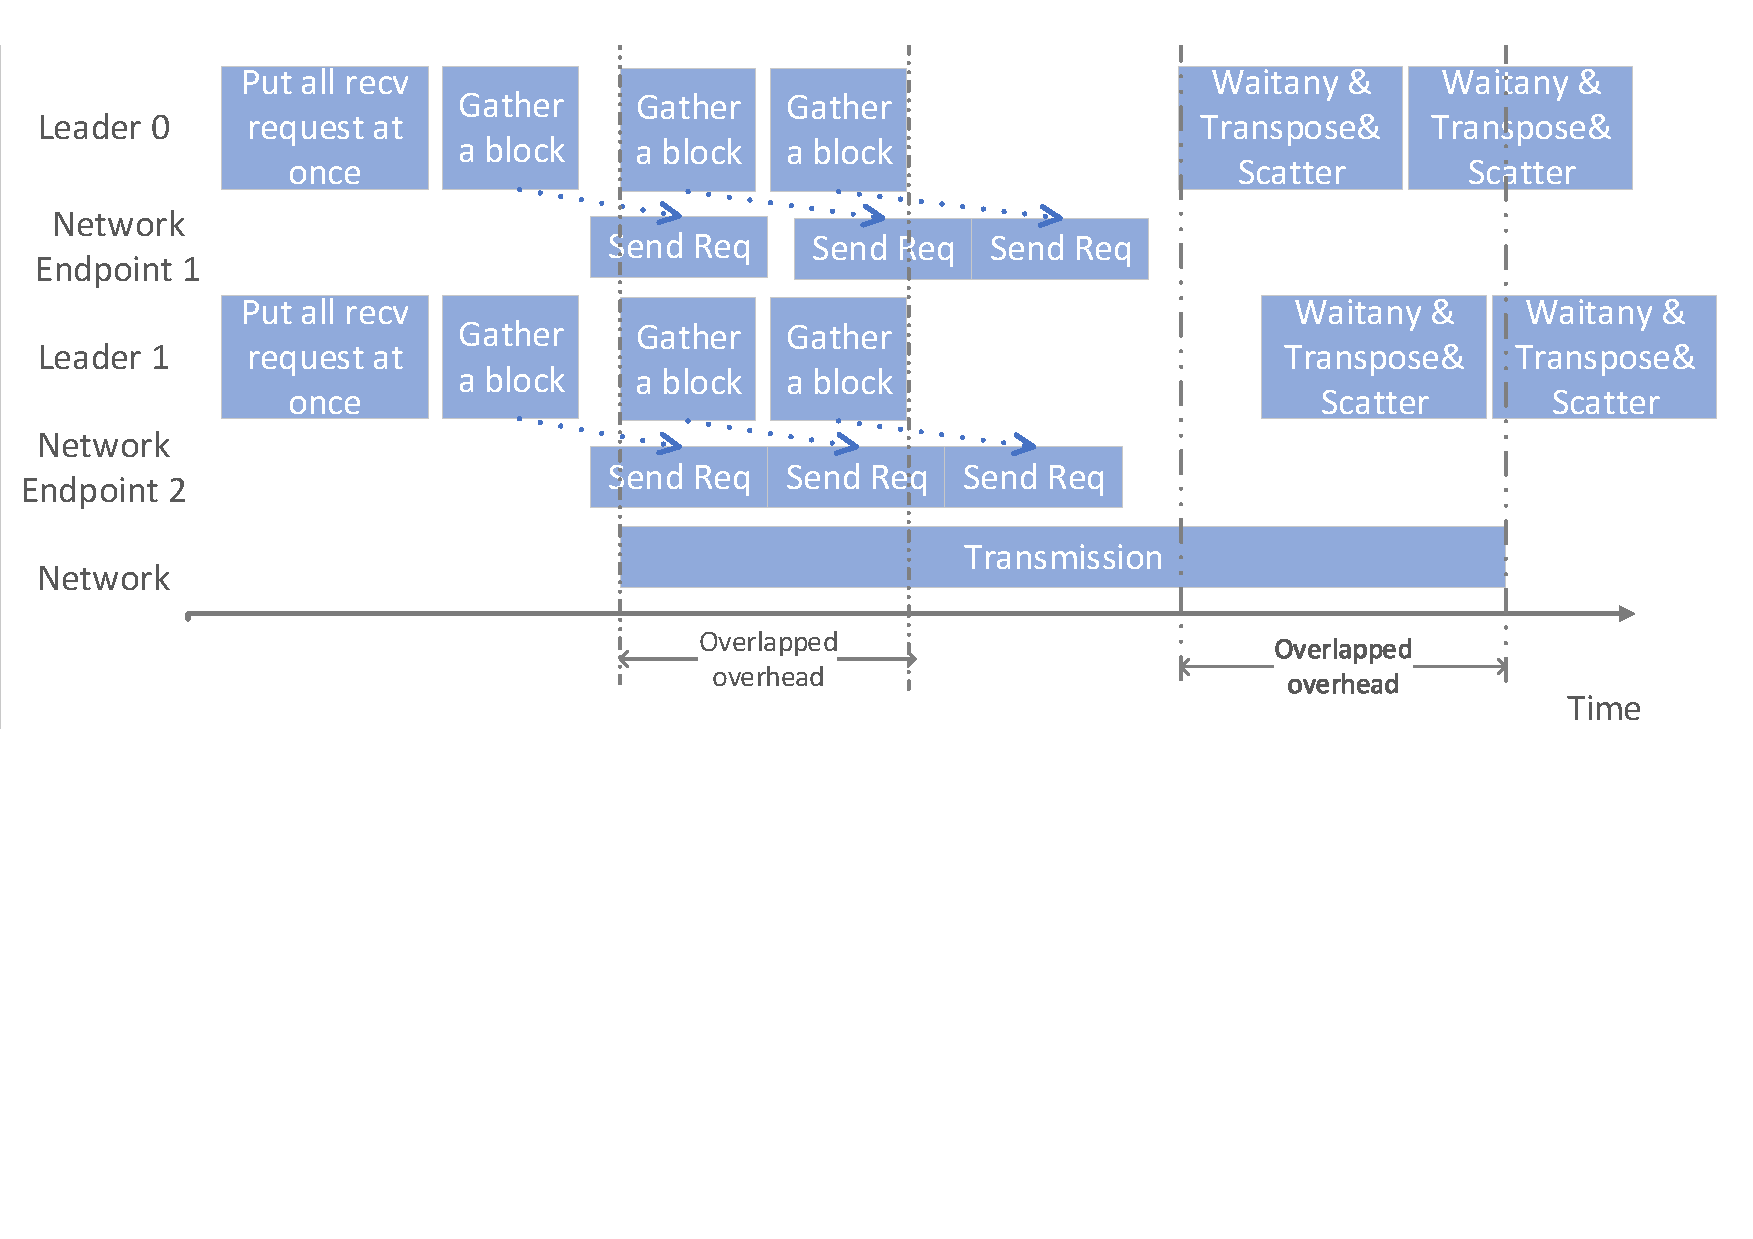
\includegraphics[width=16cm]{./Figures/Overlap-inter-intra-node-communication.pdf} %[图片大小]{图片路径}
\caption{Overlap the intra-node communication and inter-node communication with 2 leaders} %图片标题
\label{fig:ONMPML}
\end{figure*}

In Figure \ref{fig:ONMPML}, assume there are 2 leaders and 2 endpoints in a node. 
First, each leaders post all non-blocking receive requests at once.
Then, each leader start gathering data, once a block is aggregated, it sends out the block immediately.
After the first gathering, the second gathering is overlapped with network communication.
As a result, as long as the number of node is big enough, the gathering overhead can be mostly overlapped with inter-node communiation.
As to the scattering overhead, receive leaders start scattering as long as it receive one block.
While in NMPML, receive leaders start scattering data after all blocks arrived.
The throughput of ONMPML depends on  the slowest one: network bandwidth or gather-scattering throughput.

The Algorithm \ref{OverlapedMulti-leader-based-a2a} show the ONMPML algorithm on RMA (intra-node communication) and RDMA (inter-node communication).
Compared to NMPML, ONMPML using nonblock communication (MPI\_Isend/Irecv or RDMA etc.) to overlap the network communication with gathering and scattering procedure.
For gathering and scattering procedure, only leader processes are activated other processes do not participate gathering or scattering.
Remote Memory Access (RMA) makes the leaders can access other processes space directly.

\begin{algorithm}
	\caption{Overlapped NUMA-aware Multi-port Multi-leader a2a (ONMPML)}\label{OverlapedMulti-leader-based-a2a}
	\SetAlgoLined
	\KwIn{PPN:processes per-node, intra-rank: rank within a node, inter-rank: index of nodex
	}
	\SetKwProg{Def}{def}{:}{}

	\Def{all-to-all(SendBuf,RecvBuf,count,type,comm)}
	{
		intra-node-barrier()
		
		\If{am-i-leader(intra-rank)}
		{
			Lid = my-leader-id(intra-rank)

			\For{i in range(Lid,nodeN,LeaderN)}
			{
				target-node $\leftarrow$ (inter-rank + i) mod nodeN

				k $\leftarrow$ $\frac{i}{LeaderN}$

				shift $\leftarrow$ target-node*count*PPN

				\For {j in range(0,PPN)}
				{
					source $\leftarrow$ (intra-rank + j) mod P

					Get(gatherbuf[k][source],source,shift)
				}

				RDMA\_req.target $\leftarrow$ target

				RDMA\_req.event $\leftarrow$ [inter\_rank, k]

				RDMA\_Put(gatherbuf[k],RDMA\_req)
				% 
			}
			\For{i in range(Lid,nodeN,LeaderN)}
			{
				WaitAnyEvent(\&event)

				source-node $\leftarrow$ event[0]

				k $\leftarrow$ event[1]

				LocalTranspose(BufferR[k])


				shift $\leftarrow$ source-node*count*PPN

				\For {j in range(0,PPN)}
				{
					target $\leftarrow$ (intra-rank + j) mod P

					Put(BufferR[k][target],target,shift)
				}


			}
		}
		
		intra-node-barrier()
	}
\end{algorithm}


% Tianhe's RDMA operation provide a capability to control the on going messages number at the same time.
% If we set the ongoing message number to 2, each node can process a communication request as long as there is 0 or 1 requests on going.
% Lesser ongoing message number, the scattering overhead can be better overlapped with communication.
% Because messages arrives more sequentially.